\documentclass[german,a4paper, 12pt]{llncs}
\usepackage[left=30mm,right=30mm,top=25mm,bottom=25mm]{geometry}
\setlength{\footskip}{6mm} % Abstand Seitenzahl zu Text
\setcounter{tocdepth}{2}
\makeatletter
\renewcommand*\l@author[2]{}
\renewcommand*\l@author[2]{}
\makeatletter
\usepackage[utf8]{inputenc}
\usepackage[backend=biber,sorting =none]{biblatex}
\usepackage{csquotes}
\usepackage{graphicx}
\usepackage{babel}

\usepackage{parskip}
\usepackage{float}

%\usepackage{hyperref}
\usepackage{filecontents}


\begin{filecontents}{references.bib}
	
	@article{introToCNN,
		author = {O'Shea, Keiron and Nash, Ryan},
		year = {2015},
		month = {11},
		pages = {},
		title = {An Introduction to Convolutional Neural Networks},
		journal = {ArXiv e-prints}
	}
	@article{surveyOfDeepLearing,
		author = {Jiao, Licheng and Zhang, Fan and Liu, Fang and Yang, Shuyuan and Li, Lingling and Feng, Zhixi and Qu, Rong},
		year = {2019},
		month = {09},
		pages = {1-1},
		title = {A Survey of Deep Learning based Object Detection},
		volume = {PP},
		journal = {IEEE Access},
		doi = {10.1109/ACCESS.2019.2939201}
	}
	
	@ONLINE{spatialMapping,
		title = {Spatial Mapping},
		url = {https://docs.microsoft.com/de-de/windows/mixed-reality/spatial-mapping},
		urldate = {2020-04-17},
	}
	
	@ONLINE{spatialMappingUnity,
		title = {Räumliche Zuordnung in Unity},
		url = {https://docs.microsoft.com/de-de/windows/mixed-reality/spatial-mapping-in-unity},
		urldate = {2020-04-17},
	}
	
	@INPROCEEDINGS{cNNforClass,
		author={N. {Jmour} and S. {Zayen} and A. {Abdelkrim}},
		booktitle={2018 International Conference on Advanced Systems and Electric Technologies (IC ASET)}, 
		title={Convolutional neural networks for image classification}, 
		year={2018},
		volume={},
		number={},
		pages={397-402},}
	
	%https://docs.microsoft.com/de-de/learn/modules/analyze-images-computer-vision/2-image-analysis-azure
	
	@ONLINE{getAzure,
		title = {Microsoft Azure Computer Vsion},
		url = {https://azure.microsoft.com/en-us/services/cognitive-services/computer-vision/},
		urldate = {2020-06-12},
	}
	@ONLINE{whatIsAzure,
		title = {What is Computer Vision},
		url = {https://docs.microsoft.com/en-us/azure/cognitive-services/computer-vision/home},
		urldate = {2020-06-12},
	}
	@ONLINE{objDetectAzure,
		title = {Detect common objects in images},
		url = {https://docs.microsoft.com/en-us/azure/cognitive-services/computer-vision/concept-object-detection},
		urldate = {2020-06-12},
	}
	
	@ONLINE{pytorch,
		title = {From research to production},
		url = {https://pytorch.org/},
		urldate = {2020-06-12},
	}
	@ONLINE{Azure302Doc,
		title = {Mr und Azure 302 Maschinelles Sehen},
		url = {https://docs.microsoft.com/de-de/windows/mixed-reality/mr-azure-302},
		urldate = {2020-06-12},
	}
	@ONLINE{Azure302bDoc,
		title = {Mr und Azure 302b benutzerdefinierte Vision},
		url = {https://docs.microsoft.com/de-de/windows/mixed-reality/mr-azure-302b},
		urldate = {2020-06-12},
	}
	@INPROCEEDINGS{cars,
		author={X. {Chen} and H. {Ma} and J. {Wan} and B. {Li} and T. {Xia}},
		booktitle={2017 IEEE Conference on Computer Vision and Pattern Recognition (CVPR)}, 
		title={Multi-view 3D Object Detection Network for Autonomous Driving}, 
		year={2017},
		volume={},
		number={},
		pages={6526-6534},
	}
	@ONLINE{mlluminfeatures,
	title = {Magic Leap Features},
	url = {https://developer.magicleap.com/en-us/learn/guides/magic-leap-features},
	urldate = {2020-09-18},
	}
	@ONLINE{mlluminOS,
	title = {Lumin OS Overview},
	url = {https://developer.magicleap.com/en-us/learn/guides/lumin-os-overview},
	urldate = {2020-09-18},
}
	@ONLINE{mlluminOS,
	title = {Lumin OS Overview},
	url = {https://developer.magicleap.com/en-us/learn/guides/lumin-os-overview},
	urldate = {2020-09-18},
}
	@ONLINE{mlluminworldreconstruktion,
	title = {World Reconstruktion},
	url = {https://developer.magicleap.com/en-us/learn/guides/world-reconstruction-overview-landing},
	urldate = {2020-09-18},
}
	@ONLINE{mlmeshingunity,
	title = {1.4 Spatial Meshing - Unity},
	url = {https://developer.magicleap.com/en-us/learn/guides/meshing-in-unity},
	urldate = {2020-09-18},
}
	@ONLINE{mlappsecurity,
	title = {App Security},
	url = {https://developer.magicleap.com/en-us/learn/guides/application-security-overview},
	urldate = {2020-09-18},
}
	@ONLINE{mlofficialsalespitch,
	title = {magic leap 1},
	url = {https://www.magicleap.com/en-us/magic-leap-1},
	urldate = {2020-09-18},
}
	@ONLINE{mlglossary,
	title = {Glossary and Usage},
	url = {https://developer.magicleap.com/en-us/learn/guides/glossary},
	urldate = {2020-09-18},
}

	@ONLINE{unitycameratoworldmatrix,
	title = {Camera.cameraToWorldMatrix},
	url = {https://docs.unity3d.com/ScriptReference/Camera-cameraToWorldMatrix.html},
	urldate = {2020-09-18},
}

	@ONLINE{unitymultiplyoint,
	title = {Matrix4x4.MultiplyPoint},
	url = {https://docs.unity3d.com/ScriptReference/Matrix4x4.MultiplyPoint.html},
	urldate = {2020-09-18},
}
	
\end{filecontents}

\addbibresource{references.bib}
\title{Bachelorarbeit}
\subtitle{Automatisches Labeln von Objekten in einer Augmented Reality Umgebung}
\author{\parbox{.9\textwidth}{\centering 
		\large Janelle Pfeifer \\
		\small Delpstraße 28\\
		53359 Rheinbach \\
		janelle.pfeifer@smail.inf.h-brs.de}}
\institute{\parbox{.9\textwidth}{\centering 
		\large Hochschule Bonn-Rhein-Sieg \\
		\normalsize Institute of Visual Computing \\ 
		\small Fachbereich Informatik \\
		Studiengang: Informatik (B.SC.)\\
		\phantom{.}\\
		\normalsize Erstprüfer: Prof. Dr. Ernst Kruijff\\
		\normalsize Zweitprüfer: Prof. Dr. André Hinkenjann\\
		\phantom{.}\\
		\normalsize Rheinbach, 1.10.2020}}
\begin{document}
	
	%{\let\newpage\relax\maketitle}
	\maketitle
	\newpage
	\tableofcontents
	\newpage

\section{Zusammenfassung}
\section{Einleitung}
%noch ein bsichen lang. kann die beschreibung der zwei schlechteren methoden verkürzen. Abschnitte 2 3 4 

Augmented Reality (AR) ist eine Vermischung der realen Welt mit digitalen Elementen. Es wird durch Anzeigegeräte, wie Handys, Tablets oder Augmented Reality Brillen präsentiert und bietet ein intuitives Benutzerinterface um Informationen über Objekten der realen Welt anzuzeigen. Dafür müssen Informationen über die Umgebung erfasst werden. Es ist wichtig zu bestimmen welche Objekte sich in der Umgebung befinden, die durch AR erweitert werden soll.

%wie wird objekt erkennung gemacht
Es gibt mehrere Möglichkeiten reale Objekte zu erkennen. Zum einen können Markierungen in der realen Welt verwendet werden. Dabei handelt es sich um statische Bilder, beispielsweise ein Foto, oder ein QR Code, die von einer Kamera eingescannt werden. Der Marker ist einzigartig für jedes Object, das erkannt werden soll, damit sie voneinander unterschieden werden können. Der Nachteil bei diesem Vorgehen ist der Arbeitsaufwand, der damit verbunden ist, jeden Gegenstand einzeln zu Markieren und der AR Applikation die Marker bekannt zu machen. 
%Außerdem können Marker leicht verdeckt werden und nicht an jedes Object lassen sich Marker anbringen. 

Wenn man Markierungen in der Realen Welt umgehen möchte, kann man den Nutzer der Applikation bitten, per Geste oder per eye sight auf Objekte der Realen Welt zu weisen, die erkannt werden sollen. Dabei muss von dem Nutzer auch angegeben werden, um welches Object es sich genau handelt, damit die Applikation unterschiedliche Objekte auseinander halten kann und die korrekten Informationen mit ihren assoziiert. Auch hier ist ein hoher Arbeitsaufwand damit verbunden alle Objekte für die Application auszuweisen. 

%also basically per hand. was ziemlich schlecht ist. % es bleibt nur übrig automatisch zu tracken
Beide der Verfahren sind nicht auf große AR Umgebungen skalierbar, da sie sehr Arbeitsintensiv sind. Nur eine voll automatische Objekterkennung ist skalierbar. 

%object detection funktoniert was bilder angeht.
Um diese Automatisierung zu erreichen kann Image based Object Detection aus dem Bereich der Computer Vision verwendet werden.
Dabei werden Objekte in Bildern erkannt, indem nach Charakteristiken gesucht werden, die unterschiedliche Arten an Objekten auszeichnen.\cite{introToCNN}

%Diese Automatisierung wollen wir in dieser Thesis mit einer Hololens durchführen. quasi zeigen das es geht.
In dieser Thesis wird das Erkennen und Labeln von Objekten in einer AR Umgebung, mithilfe von Image based Objekt Detection, automatisiert. 
Dabei wird as AR Gerät "Magic Leap" verwendet. 


\section{Grundlagen}

\subsection*{Object Detection}
Objekt Detection ist eine Aufgabe in Computer Vision bei der Objekte in einem Bild identifiziert werden. Es wird bestimmt um welche Klasse an Objekt es sich handelt, beispielsweise ob es eine Katze oder ein Hund ist, und wo sich das Objekt befindet. Die Ausgabedaten dieser Untersuchung ist eine Liste an Objektarten und eine Liste an Bounding Boxen, die die Positionen angeben.

Object Detection kann mit Artificial Neural Networks durchgeführt werden.  

\subsection*{Artificial Neural Networks}
Artificial Neural Networks sind Machine Learning Architekturen. Sie können beispielsweise Musik, Text oder Bilder nach Mustern durchsuchen. Sie sind für keine genaue Aufgabe programmiert, sondern lernen indem sie mit Beispieldaten trainiert werden. Für jedes Beispiel gibt es ein Label, das angibt ob es das gesuchte Muster enthält oder nicht. Die Struktur des Networks verfügt über Gewichte, die Einfluss auf den Output haben. Mit jedem Trainingsbeispiel passt das Network die Gewichte an, sodass der Output dem Label des Beispiels entspricht.\cite{introToCNN,surveyOfDeepLearing}

%Artificial Neural Networks bestehen aus einer Menge an verbundenen Knoten, die jeweils eine Berechnung durchführen. Diese Knoten sind in Ebenen aufgeteilt, den Input Layer, den Output Layer, und mehrere Hidden Layer dazwischen. Die Knoten einer Ebene sind mit allen Knoten der Vorherigen Ebene verbunden.\cite{introToCNN,surveyOfDeepLearing}
%Das Neural Network bekommt eine Menge an Daten als Input. Die Knoten arbeiten zusammen um den Output zu erzeugen. Dabei wird über Gewichte entschieden, wie viel Einfluss das Ergebnis der einzelnen Knoten auf die nächste Ebene hat.\cite{introToCNN,surveyOfDeepLearing}
%Um ein Neural Network zu trainieren, wird der Output von einem Mensch bewertet. Das Neural Network nutzt diese Bewertung, um die Gewichte der einzelnen Knoten zu verändern. So passt sich das Neural Network an. \cite{introToCNN,surveyOfDeepLearing}

\subsection*{Convolutional Neural Networks}
Convolutional Neural Networks sind auf das Verarbeiten von Bildern spezialisiert. Sie nutzen aus, das Bilder viele Redundanzen und Informationsarme Bereiche haben, indem sie mit jedem Verarbeitungsschritt Informationen weglassen. So können Rechenzeit und Trainingsdaten verringert werden.\cite{introToCNN,surveyOfDeepLearing,cNNforClass}

%So wird das Convolutional Neural Network gezwungen sich auf wesentliche Teile des Bildes zu knozentrieren. Mit jedem verarbeitungsschritt sinkt die Menge an Informationen, die Das Sie Brauceh weniger Rechenzeit und weniger Trainigsdaten als ein generelles Artificial Neural Network werden eingesetzt um Muster in Bildern zu erknenne

%Convolutional Neural Networks sind Machine Learning Architekturen, die darauf ausgelegt sind, Muster in Bildern zu erkennen. Sie müssen auf das Muster trainiert werden. Dazu wird ihnen eine Menge an Bildern, die Teilweise das Muster erhalten, und der gewünschte Output, der erreicht werden soll, gegeben. Die Struktur des Network verfügt über Gewichte, die die Berechnung des Outputs beeinflussen. Mit jedem Trainigsbild passt das Network die Gewichte an, damit es die Mustern korrekt erkennen kann.\cite{introToCNN,surveyOfDeepLearing}

%Convolutional Neural Networks werden hauptsächlich eingesetzt um Muster in Bildern zu erkennen. Daher ist ihre Struktur und ihre Arbeitsweise auf Bilder spezialisiert. Sie brauchen weniger Rechenzeit und weniger Trainingsdaten als ein generelles Artificial Neural Network für dieselbe Aufgabe brauchen würde.\cite{introToCNN,surveyOfDeepLearing,cNNforClass} 
%Die Knoten in einer Ebene eines Convolutional Neural Network sind nur mit wenigen Knoten der vorherigen Ebene verbunden. So sinkt die Menge an Informationen mit jeder Ebene. Das CNN wird gezwungen sich auf wesentliche Teile des Bildes zu konzentrieren, mit denen beispielsweise ein Objekt oder  Muster erkannt werden kann. \cite{introToCNN,surveyOfDeepLearing}

\subsection*{Azure maschinelles Sehen}
Microsoft Azure bietet einen Computer Vision Service an, der für Object Detection trainiert ist.
Der Anwender sendet ein Bild an Microsoft, dort wird es verarbeitet und ein Ergebnis zurückgegeben.\cite{getAzure,whatIsAzure,objDetectAzure,Azure302Doc}

Der Service wird über einen web request angefragt. Und sendet eine Json Datei zurück. 

Über ein web endpoint per web request anfragen. Bekommt eine Json zurück. darin steht welche Obejkte darin sind, daten über das foto und objekte mit bounding box angegeben. Beispiel von Json angeben. 

%todo write more about this
\subsection*{Azure Custom Vision}
Azure bietet zusätzlich einen Computer Vision Service an, den der Nutzer Trainieren kann um bestimmte Objekte Klassifizieren zu können.\cite{Azure302bDoc}

was ist die Prediction? 
Erkälre die Iterations
Erkläre was die Genauigkeit der Predation aussagt.
%todo write more about this
\subsection*{Spatial Mapping} 
Durch Spatial Mapping wird eine 3D Abbildung einer realen Umgebung erschaffen. So können Hologramme mit der echten Welt interagieren, diese Verdecken, oder von ihr verdeckt werden.\cite{spatialMapping} 

\subsection*{Magic Leap AR Brille}

Die Magic Leap 1 Lightwear ist eine Augmented Reality Brille. Sie besitzt neun Sensoren und mehrere Kameras. Dazu gehören:
\begin{itemize}
	\item ein Infrarot Tiefen-Sensor,
	\item ein Eye Tracker,
	\item eine Foto und Video Kamera, die im Format 16:9 mit einer Auflösung von 1920 x 1080 Pixeln aufnehmen,
	\item Umgebungskameras die in unterschiedliche Richtungen ausgerichtet sind. \cite{mlofficialsalespitch,mlglossary}
\end{itemize}

Output geschieht über ein Display mit einem 50 Grad Field of View und einem Seitenverhältnis von 4:3. 
Input wird durch ein 6 Degree of Freedom Controller gegeben.\cite{mlofficialsalespitch,mlglossary}

Die Magic Leap Brille läuft auf dem Betriebssystem Lumin OS. Dieses wurde für Spatial Computing entwickelt und stellt Applikationen entsprechende Funktionalitäten zur Verfügung.
Beispielsweise führt das Betriebssystem Spatial Mapping durch. Mit den Sensoren und Kameras der Brille werden Daten aufgenommen und in einen Zeitlichen Zusammenhang mit der Bewegung der Brille gesetzte, um eine Rekonstruktion des Raumes zu erhalten.\cite{mlluminOS,mlluminfeatures,mlluminworldreconstruktion,mlmeshingunity}

Lumin OS bietet es Applikationen an,
\begin{itemize}
	\item Raycast auf die Umgebung durchzuführen und
	\item ein Mesh der Rekonstruktion zu erhalten.
\end{itemize}

Lumin OS unterstützt das Verarbeiten von dem Input des Controllers und verwaltet die Privilegien der Applikationen. Dazu gehört beispielsweise der Zugriff auf die Fotokamera und das Netzwerk.\cite{mlluminfeatures,mlappsecurity}
\subsection{Webrequests}

%todo: this
%hmmm do I have to explain this ?

\subsection*{3D-Computergrafik}
\subsection{Lokale und globale Koordinatensysteme in 3D Szenen}

In einer 3D Szenen werden die Positionen von Objekten als Matrizen in drei Dimensionalen Koordinatensystemen verwaltet.
Es gibt ein globales Koordinatensystem (auch Weltkoordinatensystem oder World Space), in dem alle Objekte relativ zu einem gewählten Ursprung liegen. 

Jedes Objekt hat zusätzlich ein eigenes, lokales Koordinatensystem (Objektkoordinatensystem). Dessen Ursprung liegt in dem jeweiligen Objekt.
Die Position und Rotation des Objektes in dem globalen Koordinatensystem bestimmt die Relation zwischen dem globalen und dem lokalen Koordinatensystem. 

Das lokale Koordinatensystem einer Kamera wird auch Camera Space genannt. Die Relation zwischen dem Camera Space und dem globalen Koordinatensystem wird in Unity durch die cameraToWorld Matrix beschrieben. Mithilfe dieser Matrix kann eine Koordinate aus dem Camera Space in die entsprechende Koordinate des globalen Koordinatensystems transformiert werden.\cite{unitycameratoworldmatrix}

Dazu wird die Koordinate als Vektor angegeben und mit der cameraToWorld Matrix multipliziert. Das Resultat ist ein Vektor, der eine Koordinate im globalen Koordinatensystem angibt.\cite{unitycameratoworldmatrix,unitymultiplyoint}

\subsection{Kamera in 3D-Computergrafik}
\subsubsection{View Frustum}
ist der Teilvolumen einer 3D Szene, die auf den zweidimensionalen Bildschirm abgebildet wird. Alle Objekte die von der Kamera gesehen werden, befinden sich in dem View frustum.

\subsubsection{Clipping Plane}
bezeichnet eine Ebene, die den view frustum quer zur Blickrichung begrenzt. 
Es gibt eine vordere und eine hintere Clippingebene.
Die vordere Clippingebene liegt nahe an der Kamera dran. Alle Objekte die zwischen der Kamera und der Ebene liegen werden nicht angezeigt.

Die hintere Clippingebene limitiert wie weit Objekte entfernt sein können, bevor sie nicht mehr zu sehen sind.

%to myself: yay :) you're doing well I believe in you!

\section{Design}
Das Ziel ist das Erkennen und Labeln von Objekten in einer AR Umgebung, durch Image Based Objekt Detection.

Wenn der Nutzer das Signal gibt, beginnt die Detection. Als Erstes wird ein Foto mit der Kamera der AR Brille aufzunehmen. 
Dieses Foto wird dann an Azure Object Detection und Azure Custom Vision geschickt. 
Als Ergebnis gibt es jeweils eine Json Datei. Darin wird angegeben, welche Arten von Objekten auf dem Foto gefunden wurden (Hund, Person, Computermaus) und wo sie sich jeweils befinden. Die Position eines Objektes ist dabei mit einer Bounding Box bestimmt. Um das Markieren von Objekten in der AR Umgebung zu vereinfachen, wird die Mitte der Box als Position des Objektes genommen.

Jedes Objekt soll an der tatsächlichen Stelle der Realen Welt markiert werden.
Dafür wird in der 3D Szene der AR Umgebung eine Virtuelle Repräsentation des Fotos erschaffen. Die Fotorepräsentation muss die richtige Skalierung, Position und Rotation haben, um das räumliche Verhältnis zwischen der realen Foto-Kamera und der Umgebung nachzubilden.

Da die Foto-Kamera und das Display nahe beieinander liegen und den gleichen Blickwinkel haben, kann die Position des Displays als Repräsentation des Fotos genutzt werden. In der 3D Szene ist das Display mit der Hauptkamera gleichgesetzt. Die Clipping Plane der Kamera hat somit die gleiche Rotation und eine zumindest ähnliche Position und Skalierung wie das Foto. 

Daher werden die Foto-Positionen auf Koordinaten der Clipping Plane abgebildet. Dabei werden verbleibende Positions- und Skalierungs-Unterschiede ausgeglichen. Für jedes Objekte wird so eine Koordinate auf der Clipping Plane bestimmt. 

Als Nächstes wird ein Raycast von der Kamera aus durch die Clipping Plane Koordinate geschickt. Der Raycast schneidet sich mit einem Mesh, das die reale Welt abbildet. Die getroffene Position wird mit einem Schriftzug markiert. Dort befindet sich das Objekt, das auf dem Foto gefunden wurde.

Alle Objekte, die Azure Object Detection und Azure Custom Vision gefunden haben, werden so für den Nutzer in der AR Umgebung markiert.

\section{Implementierung}
% https://developer.magicleap.com/en-us/learn/guides/get-started-developing-in-unity
Das Projekt wurde in Unity umgesetzt, und wurde für eine Magic Leap AR Brille entwickelt.
Es wurde ein Unity Projekt Template von Magic Leap verwendet. 

Zusätzlich werden einige vorgefertigte Klassen von Magic Leap verwendet. Dazu gehören MLInput, MLCamera, MLRaycast, MLPrivilegeRequestBehavior und MLSpatialMapper.

MLSpatialMapper setzt spatial mapping um und erzeugt ein Mesh, das die Umgebung abbildet.
%\subsection{Input}

%Der Input des Controllers wird in der Klasse InputHandler verarbeitet. Die Klasse MLInput verwaltet den Status des Controllers. In InputHandler werden die Stadi interpretiert und Mithilfe von MLInput werden ButtonDown und ButtonUp events abgefangen. 

\subsection{Ein Foto aufnehmen}

Das Script TakePicture implementiert das aufnehmen von einem Foto.
Die Methode StartCapture wird aufgerufen, um den Process zu starten. 
MLCamera wird genutzt um die Kamera der Magic Leap Brille anzusteuern.

%Image: Aufgenommenes Foto wird in AR UI angezeigt.

Wenn das Foto uafgenommen wurde, wird OnCaptureRawImageComplete aufgerufen. Die Daten des Bildes werden an die Klassen Azure ObjectDetection und AzureCustomPrediction weitgergegeben. Dort wird die Analyse der Bilder gestartet. 

\subsection{Azure Object Detection}

In der Methode AnalyseImage von AzureObjectDetection wird ein Web Request zusammengestellt. Azure stellt dafür einen Web endpoint zur verfügung. In dem Request muss ein Authorization Key für den Service und die Bild-Daten enthalten sein.

Der Webrequest wird geschickt und es wird auf die Antwort gewartet. Wenn es keine Probleme mit dem Netzwerk gab, wird eine JsonDatei als String in der Antwort auf den Webrequest geschickt. Siehe Abbilung ??

%todo picture of a json response. 

Es wird für jedes gefundene Object auf dem Foto eine Bezeichnung und eine Bounding Box angegeben, in dem sich das Object auf dem Bild befindet. 

Die Json Datei wird in HandleJsonResponse verarbeitet. Für den erwarteten Aufbau der Datei wurden drei Klassen geschrieben. Der Json String wird mit JsonUtility in ein DetectionResponse Object umgewandelt. Dabei werden alle gefundenen Foto-Objekte in einer Liste von DetectedObject abgelegt. %https://docs.unity3d.com/ScriptReference/JsonUtility.FromJson.html

Die Gefundenen Object sollen im 3D Raum mit einer Markierung ausgezeichnet werden. 
Dafür wird für jedes DetectedObject die Methode Cast von der Klasse PixelToWorld aufgerufen. Der Methode wird der Mittelpunkt der BoundingBox als u,v Foto-Koordinate für das DetectedObject übergeben.

\subsection{Von dem Foto zum 3D Raum}

In der Methode Cast wird die u,v Foto-Koordinate des Fotos und die Kameraausrichtung verwendet um das gefundene Foto-Objekt in der 3D Abbildung der Realen Welt zu lokalisieren.

Das Foto kann mit dem Display und somit mit der Clipping Plane der Hauptkamera approximiert werden.
Die u,v Foto-Koordinate wird zunächst in eine x,y,z Koordinate in dem Camera Space umgewandelt. Der z Anteil gibt die Achse an, die von der Kamera nach vorne durch den View Frustum verläuft. Bei z = -0.4 wird der Punkt auf der Achse gewählt, auf dem die Clipping Plane liegt. 

Die x und y Dimensionen beschreiben die Achsen, die horizontal und vertikal zur Clipping Plane verlaufen. Mit dem festgelegten z = -0.4, kann jeder Punkt auf der Clipping Plane durch x und y angegeben werden. Dazu gehören auch Punkte die außerhalb des View Frustum liegen.

Es wurden Werte für x und y ausprobiert, mit denen die Ränder des Fotos auf der Clipping Plane angegeben werden können. Dabei wurde darauf geachtet, das das Foto ein Seitenverhältnis von 16:9 hat, während das Display, und somit die Kamera, ein Seitenverhältnis von 4:3 hat. Darüber hinaus ist der Bildausschnitt des Displays kleiner. Daher liegen die Ränder des Fotos außerhalb des View Frustum. 

Sind die x und y Werte für die Ränder bekannt, ergibt sich für die Achsen jeweils ein Intervall, die kombiniert alle Foto-Koordinaten auf die Clipping Plane abbilden können. Die Intervall lauten: [-0.295,0.2281] für x und [0.1546,-0.1507] für y. Durch die Intervalle wird die Position und Skalierung des Fotos in Relation zu dem Display - und der Hauptkamera- berücksichtigt. Siehe Kapitel \ref{section:devpixeltoworld} für die Entwickelung des Cast Methode und die Ermittelung der Intervall Werte.

Es werden zwei Lineare Funktionen aufgestellt:
\begin{itemize}
	\item Die Funktion X Bildet das Intervall für u [0,1920] auf das Intervall für x [-0.295,0.2281] ab.
	\item Die Funktion Y Bildet das Intervall für v [0,1080] auf das Intervall für y [0.1546,-0.1507] ab.
\end{itemize}
Siehe Abbildung \ref{code:uvtoxy}.
\begin{figure}[H]
	\centering
	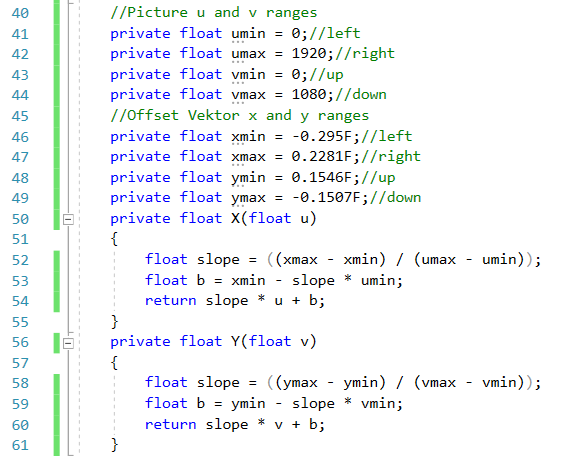
\includegraphics[width=0.6\textwidth]{images/code_uv_to_xy_scale.PNG}
	\caption[]{Funktionen X und Y}
	\label{code:uvtoxy}
\end{figure}

Mit den Funktionen wird für u,v eine Koordinate im Camera Space berechnet. Diese Koordinate wird dann mithilfe der cameraToWorldMatrix in die Koordinate p des globale Koordinatensystem umgewandelt. Damit wird die Position und Rotation der Kamera - und somit des Fotos - in der 3D Szene berücksichtigt. Siehe Abbildung \ref{code:castmethod}.

\begin{figure}[H]
	\centering
	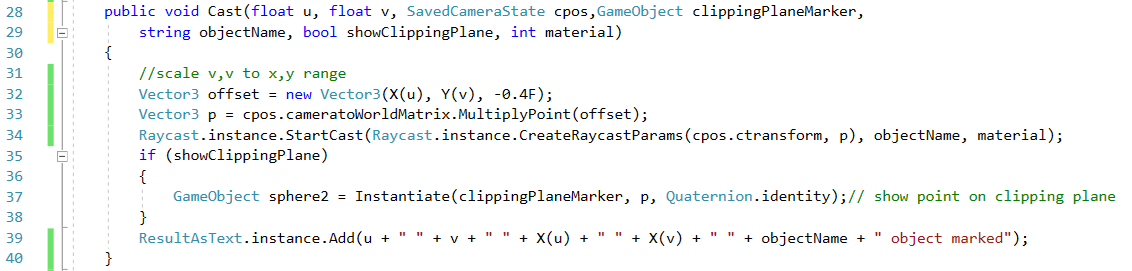
\includegraphics[width=1.2\textwidth]{images/code_cast_method.PNG}
	\caption[]{Cast Methode}
	\label{code:castmethod}
\end{figure}
\subsection{Raycast}

Als Nächstes wird ein Raycast durch den Ursprung der Kamera und die Koordinate p gesendet. MLRaycast wird genutzt, um einen Schnittpunkt mit der Rekonstitution der Welt von Lumin OS zu bestimmen. Die Stelle die der Raycast trifft beschreibt die Position des DetectedObject im 3D Raum.

Für den MLRaycast werden zwei Parameter benötigt:
\begin{itemize}
	\item Ein QueryParams Objekt, das Ursprung und Richtung für den Raycast beinhaltet.
	\begin{itemize}
		\item Ursprung: Kamera
		\item Richtung: Richtungsvektor von der Kamera zu der Koordinate p
	\end{itemize}
	\item Eine Methode die aufgerufen wird, wenn der Raycast fertig ist. 
		\begin{itemize}
		\item Callback Methode: HandleOnRecieveRaycast
	\end{itemize}
\end{itemize}

Siehe Abbildung \ref{code:raycastparams}.

\begin{figure}[H]
	\centering
	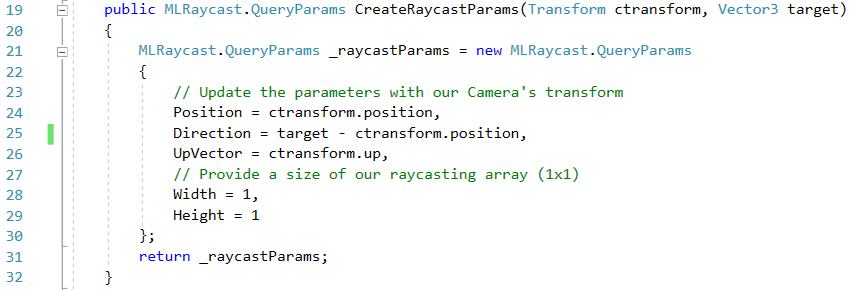
\includegraphics[width=0.9\textwidth]{images/code_raycastparams.PNG}
	\caption[]{Cast Methode}
	\label{code:raycastparams}
\end{figure}

Wenn der Raycast fertig ist, wird die Methode HandleOnRecieveRaycast aufgerufen. Der Parameter point beinhaltet dabei die getroffene Koordinate.
Diese an die Methode CreateMarker von der Klasse LabelCreater weitergegeben.

\subsection{LabelCreater}

CreateMarker erhält den Punkt point der getroffen wurde und die Bezeichnung für das DetectedObject. An der Koordinate von point wird ein Prefab GameObject instanziiert, das als Markierung für das DetectedObject in der 3D Umgebung dient.

Das Prefab besteht aus einer Kugel und einem Schriftzug, der den Namen des DetectedObject anzeigen soll. Dem neu instanziierten GameObject wird die Bezeichnung des DetectedObject als Schriftzug zugewiesen. Siehe Abbildung \ref{image:labels}.

\begin{figure}[H]
	\centering
	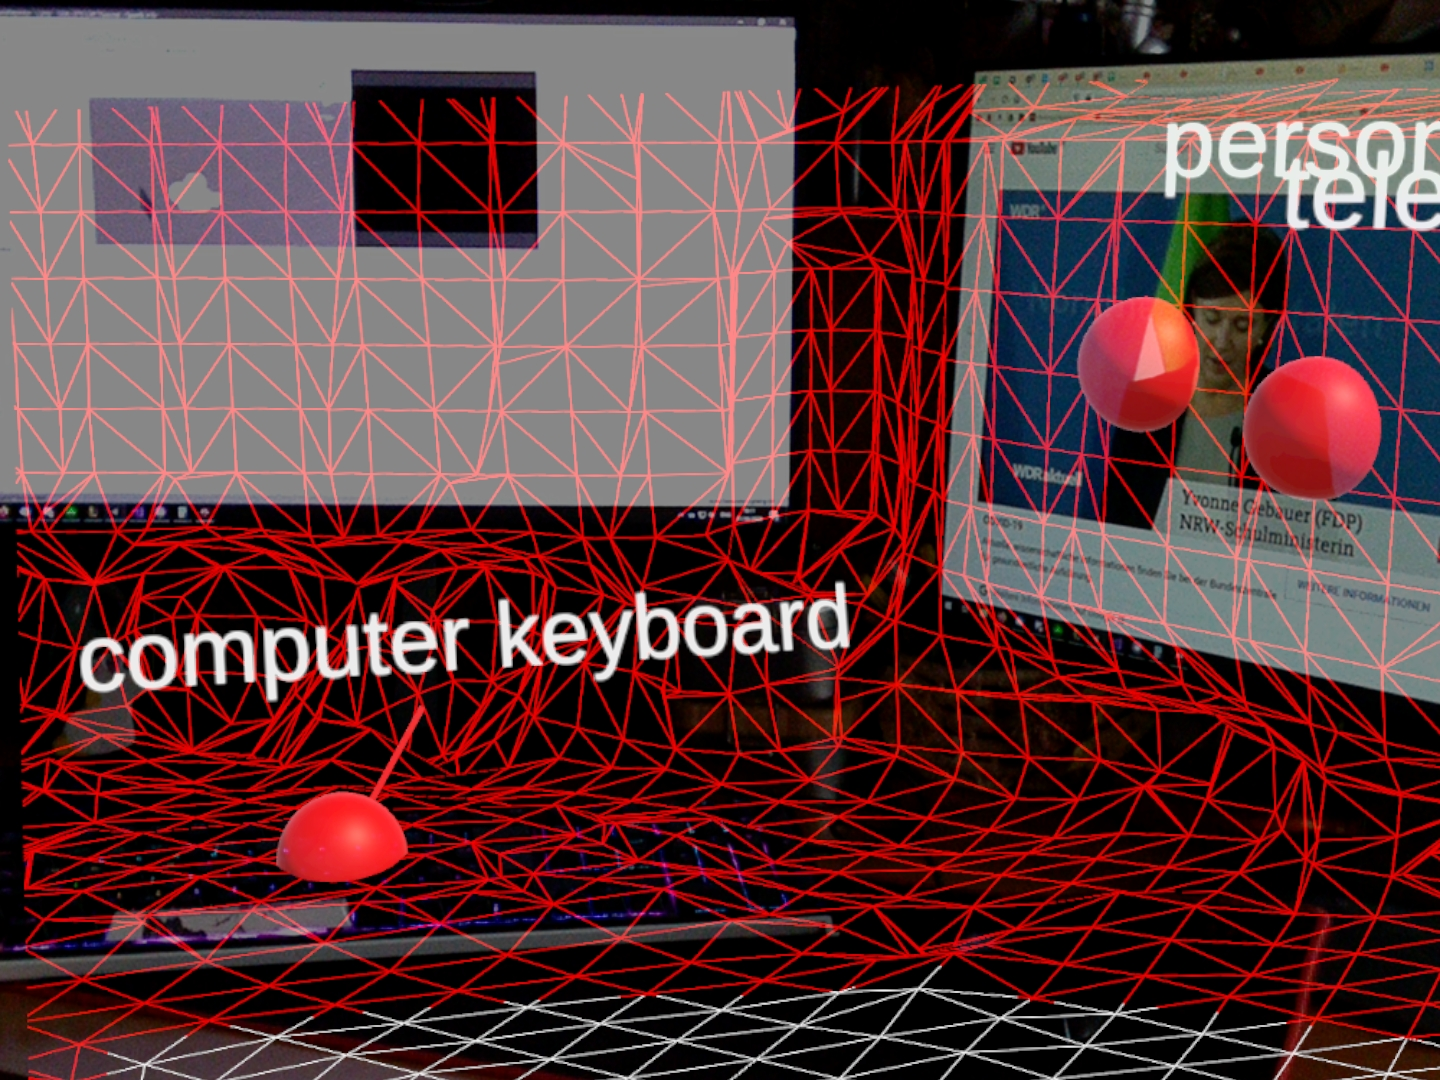
\includegraphics[width=0.7\textwidth]{images/ML_labels.jpg}
	\caption[]{Markierungen in der Welt}
	\label{image:labels}
\end{figure}

\subsection{Azure Custom Vision}

Neben der Bildanalyse mit Azure Object Detection wird auch Azure Custom Vision verwendet.
Die AI wurde über die Webseite trainiert.

Die Anfrage an den Service passiert in der Klasse AzureCustomPrediction. Ähnlich wie bei AzureObjectDetection wird ein Webrequest erstellt mit einem authorization key für den Service und einem Foto als payload.

In der Antwort wird eine Json Datei zurückgeschickt, die die gefundenen Objecte angibt.
Da die Json Datei eine etwas anderes Format hat, wurde eine eigene Handle Json Methode dafür geschrieben.

Für jedes erkannte Objekt wird die Methode Cast von PixelToWorld aufgerufen, um das Objekt in der realen Welt zu lokalisieren und zu markieren.

\subsubsection{Das Trainieren}

Es wurde Probiert das Cusotm Vision Modell auf drei unterschieldiche Objekte zu trainieren.
Dabei wurden vier Iterationen erstellt. 

Iteration 1:

Zunächst wurde probiert Tuben von Acrylfarbe zu erkennen. Die Genauigkeit war davon war nicht so gut. Es wurden in den Fotos Acrylfarben erkannt, wo es keine gab. Sieh Abbildung \ref{image:customVisionPaint}. 

\begin{figure}[H]
	\centering
	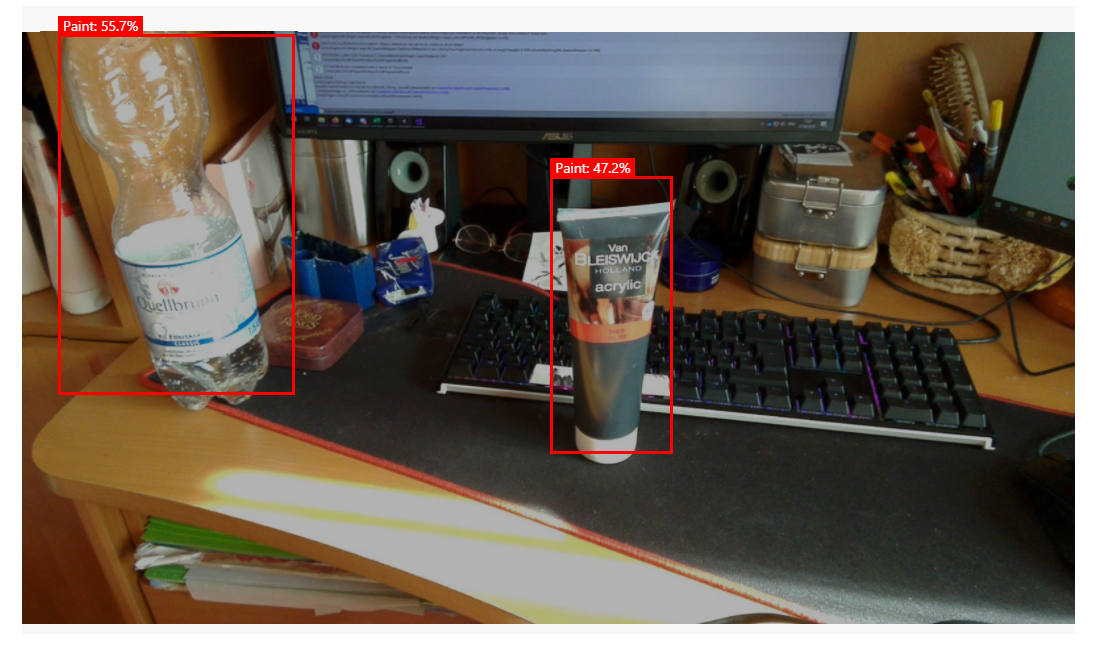
\includegraphics[width=1.0\textwidth]{images/customVisionPaint.PNG}
	\caption[]{Beispielfoto Iteration 1. Die Wasserflasche wurde als Farbe markiert mit 55.7 Prozent statistischer Konfidenz. Die Tatsächliche Farbtube wurde mit einer Konfidenz von 47.5 Prozent erkannt.}
	\label{image:customVisionPaint}
\end{figure}

Iteration 2:

In der zweiten Iteration wurde probiert das Model darauf zu trainieren, eine Blaue Dose von Nivea Hautcreme to erkennen. Die Form und Farbe von der Dose ist sehr simpel, daher wurde davon ausgegangen, das sie leicher zu erkennen ist. Auch dort dar die Genauigkeit zunächt bei nur 80 Prozent. Es wurden in vielen Fotos fälschlicherweise Nivea Dosen erkannt.

Iteration 3:

In der Iteration drei wurde versucht Iteration 2 zu verbessern. Es wurden ausgewählte Training Fotos entfernt, die die Dose von einem Seitlichen Winkel zeigten, mit der mit der Erwartung das die Detektion der Dose aus dem Blickwinkel von Oben damit konsistenter wird. Zusätzlich wurden mehr Fotos von der Dose auf verschieden farbigen und gemusterten Untergrund hinzugefügt. 

Die Genauigkeit der Prediction sank auf 75 Prozent.

Iteration 4:

In Iteration 4 wurden zwei Fotos von der Nivea Dose entfernt, das die Genauigkeit auf 100 Prozent steigen ließ. In der Umsetzung mit der Magic Leap Anwendung werden trotzdem häufig Objekte fälschlicherweise als Nivea Dose markiert.

Neben der Dose wurde diese Iteration darauf trainiert eine bestimmte Holz Haarbürste zu erkennen. Aufgrund von dem komplexeren, und markanten Aussehen der Bürste ist davon ausgegangen, das die Bürste besser von anderen Objekte zu unterschieden ist. 
Die Bürste wurde nur mit den Borsten nach oben Photographiert.

Die Genauigkeit für die Bürste lag bei 100 Prozent. 
In der Umsetzung mit der Magic Leap Anwendung wird die Bürste häufig nicht erkannt, obwohl sie im Bild ist und mit den Borsten nach oben liegt. Es werden jedoch keine Objekte als Haarbürste erkannt die keine sind.

\subsection{Entwicklung der Foto-Repräsentation}
\label{section:devpixeltoworld}
%todo verweis auf diese Section von Cast Section aus.

Um die u,v Foto-Koordinate eines gefundenen Objektes auf der Clipping Plane der Kamera zu lokalisieren wurden ein paar Herangehensweisen ausprobiert.

Das Ziel ist das setzten einer Markierung in dem 3D Raum, basierend auf der Foto-Koordinate. Das Foto beinhaltet keine Information über die Entfernung zu dem Objekt. Dafür muss ein Raycast durchgeführt werden. 

Mit einer Repräsentation des Fotos in dem 3D Raum ist es möglich ein Raycast durchzuführen. 
Dazu muss das Foto nicht tatsächlich in dem 3D Raum vorhanden sein. Es muss jedoch mit dem Input von einer Foto-Koordinate ein Output von einer Koordinate in dem 3D Raum geben, mit dem der Raycast durchgeführt werden kann.

Die Position des Fotos hängt mit der Kamera zusammen, daher kann das Foto durch den Camera Space simuliert werden. Als erstes wurde probiert ein Sphären-Objekt an eine gezielte Koordinate in dem Camera Space zu bewegen. 

% make pretty after this
Wenn die Kamera an dem Ursprung des globalen Koordinatensystem liegt und eine neutrale Rotation hat, stimmt der Camera Space mit dem globalen Koordinatensystem überein. Die Sphäre wurde in der Szene per Hand bewegt um markante Koordinaten des Camera Space abzulesen. Dabei wurden foglende Camera Space Koordinaten gefunden:
\begin{itemize}
	\item Near Clipping Plane bei z = -0.37
	\item linker Rand bei x = -0.153
	\item rechter Rand bei x = 0.153
	\item oberer Rand bei y = 0.1147
	\item unterer Rand bei y = -0.1147
\end{itemize}

Die x und y Koordinaten hängen von der u,v Koordinate des Fotos ab. Es wurden linear Funktionen aufgestellt um u,v auf x,y Abzubilden. Diese Abbildung dient als Repräsentation des Fotos im 3D Raum. Zusätzlich gibt die Position und Skalierung des Fotos im Verhältnis zu der Kamera an.

Dann wurde getestet wie genau DetectedObjects in der AR Umgebung lokalisiert werden. Es wurden Testweise Fotos aufgenommen, analysiert und die DetectedObjects markiert. Die entstandenen Markierungen lagen in Sichtfeld, jedoch nicht an den erwarteten Stellen. 

Um dem Problem auf den Grund zu gehen, wurde ein UI Objekt erstellt, das ein Aufgenommenes Foto bei Runtime anzeigt.
Das Foto wurde dann mit dem Display verglichen. Dabei viel auf, das sie ein unterschiedliches Seitenverhältnis haben und das Display einen kleinen Bildausschnitt zeigt.  

Mit den Unterschieden zwischen dem Foto und dem Display zwei Möglichkeiten. Entweder wird das Foto auf das Display zugeschnitten, oder das gesammte Foto wird genommen. Dann würden auch Objekte erkannt, die außerhalb des Sichtfeldes liegen.
es wurde die Entscheidung getroffen das Foto zuzuschneiden. Damit gibt es ein besseres Feedback für den Nutzer, das ein Objekt gefunden wurde. 

Die Zugschneidung wurde realisiert, indem die Intervalle für u und v der Abbildungsfunktionen stärker eingegrenzt wurden. Alle Objekte die Außerhalb der Intervalle liegen werden ignoriert. Um die Intervalle zu bestimmen wurde ein Gitter zu dem Fotoanzeige UI Element hinzugefügt. Mit dem Gitter kann die u,v Position von beliebigen Stellen des Fotos abgelesen werden. 
Durch aufnehmen von Fotos und vergleichen mit dem Sichtfeld des Displays wurde abgelesen, bei welcher u,v Position des Fotos sich die Ecken des Displays befinden. Die Intervalle wurden dem entsprechend eingegrenzt. 

Mit den durchgenommenen Veränderungen der Intervalle konnten DetectedObjects korrekt in der Umgebung lokalisert werden. Jedoch wurden sehr häufig Objekte nicht markiert, obwohl sie im Sichtfeld des Nutzers lagen, weil deren Mittelpunkt außerhalb eines Intervalls war.

Daher wurde entscheiden doch das gesamte Foto zu verwenden und Objekte auch zu Markieren, wenn sie komplett außerhalb des Sichtfeldes lagen. 
Dafür wurde die Intervalle für u und v wieder auf die ursprünglichen [0,1920] und [0,1080] gesetzt. Die Intervalle für x und y mussten vergrößert werden.

Um die x und y Intervalle bestimme zu können wurde das Fotoanzeige UI Element Parallel zu der ClippingPlane gelget. Das Element folgt den Bewegungen der Kamera und liegt so nah an der Near Clipping Plane wie es geht und noch angezeigt wird. Das Display der Magic Leap Brille zeigt selbst solide Objekte leicht durchsichtig an. Das wurde genutzt, um Fotos aufzunehmen, mit dem UI Element anzuzeigen und mit der Realen Welt zu vergleichen. Durch ausprobieren wurde das UI Element so skaliert und verschoben, das das Foto mit der realen Welt soweit wie möglich übereinstimmt.

Dann wurden die Ränder des UI Elementes genutzt um die Intervalle für x und y zu bestimmen.
\begin{itemize}
	\item für x: [-0.295, 0.2281]
	\item für y: [0.1546, -0.1507]
	\item Zusätzlich wurde z = -0.4 gesetzt. Das Ui Element musste ein wenig weiter von der Clipping Plane entfernt werden um angezeigt zu werden.
\end{itemize}

Mit diesen Intervallen für u,v,x und y konnten DetectedObjects gut lokalisiert werden und es wurden keine Objekte mehr weggelassen, von dennen der Nutzer erwarten würden, das sie markiert werden.


%bilder zeigen wie es dann aussieht
%make methods, classes and variables italic

\section{Zusammenfassung}
%sachen die verbessert werden könnten
%todo this part.
man kann zusätzlich zum raycast auf das mesh auch noch die tiefenkamera nutzen. spatial mapping hat manchmal das mesh an der stelle noch nicht, oder ist nicht aktualisiert. besonders probleme mit wasserflaschen die nicht erkannt werden. HInzuzihenen von tiefen datan kann das lokalisieren von objekten im 3D raum noch verbessern.
	
	\newpage
	\printbibliography
\end{document}